%% LaTeX2e class for seminar theses
%% sections/content.tex
%% 
%% Karlsruhe Institute of Technology
%% Institute for Program Structures and Data Organization
%% Chair for Software Design and Quality (SDQ)
%%
%% Dr.-Ing. Erik Burger
%% burger@kit.edu
%%
%% Version 1.0.2, 2020-05-07

\section{Basic of camera geometry}
\label{ch:basic of camera geometry}

%% -------------------
%% | Example content |
%% -------------------
The first generation of stereo-based depth estimation methods relied typically on matching pixels across multiple images captured using accurately calibrated cameras. Although these techniques can achieve good results, they are still limited in many aspects. For instance, they are not suitable when dealing with occlusions, featureless regions, or highly textured regions with repetitive patterns. We will introduce the camera geometric relationship, conventional pixel matching method and some important concept in multi-view estimation. e.g. disparity and depth. 

\subsection{camera model: projection matrix}
\label{projection matrix}
A test object introduces a characteristic modulation to the irradiated light, so that one can obtain information about the test object from the emitted light\cite{1400121}. This interactive effect can be described as simplified model called light filed $\mathcal{L}(x_{w}, \beta)$, where the process of radiance of all light rays coming from a point $x_{w}$ of the test object in the direction $\beta$ is modelled. The light field $\mathcal{L}(x_{w}, \beta)$ is a five-dimensional function of the position $x_w = (x_w, y_w, z_w)$, $T \in \mathrm{R}_3$ and the direction $\beta = (\beta_1, \beta_2)$. If $\mathcal{L}(x_{w}, \beta)$ is known for all of the surface’s points $x_w \in \mathrm{SF}$, then the light field $\mathcal{L}(x_{w}, \beta)$, $u \in \mathrm{R}_3$ induced by the test object is uniquely defined for the surrounding space. In our project, we used a completely simplified model based on the lifht field model, which has only four parameters, namly $\mathcal{L}(x_{w}, o_i, \lambda)$, where $o_i$ defines the angular information of the camera in three dimensional world and $\lambda$ represents the color perception through the microlens, in this situation $\lambda = (l_r, l_g, l_b)$. To explain this model intuitively we introduce the pinhole camera model and derive the projection matrix of a normal camera. 
\begin{equation}
\label{eqn:lf_model1}
    \mathcal{L}(x_{w}, o_i, \lambda) \quad x_w=(x_x, x_y,x_z), \quad o_1 = (o_x, o_y, o_z), \quad \lambda = (l_r,l_g,l_b)
\end{equation}

\begin{figure}
\centering
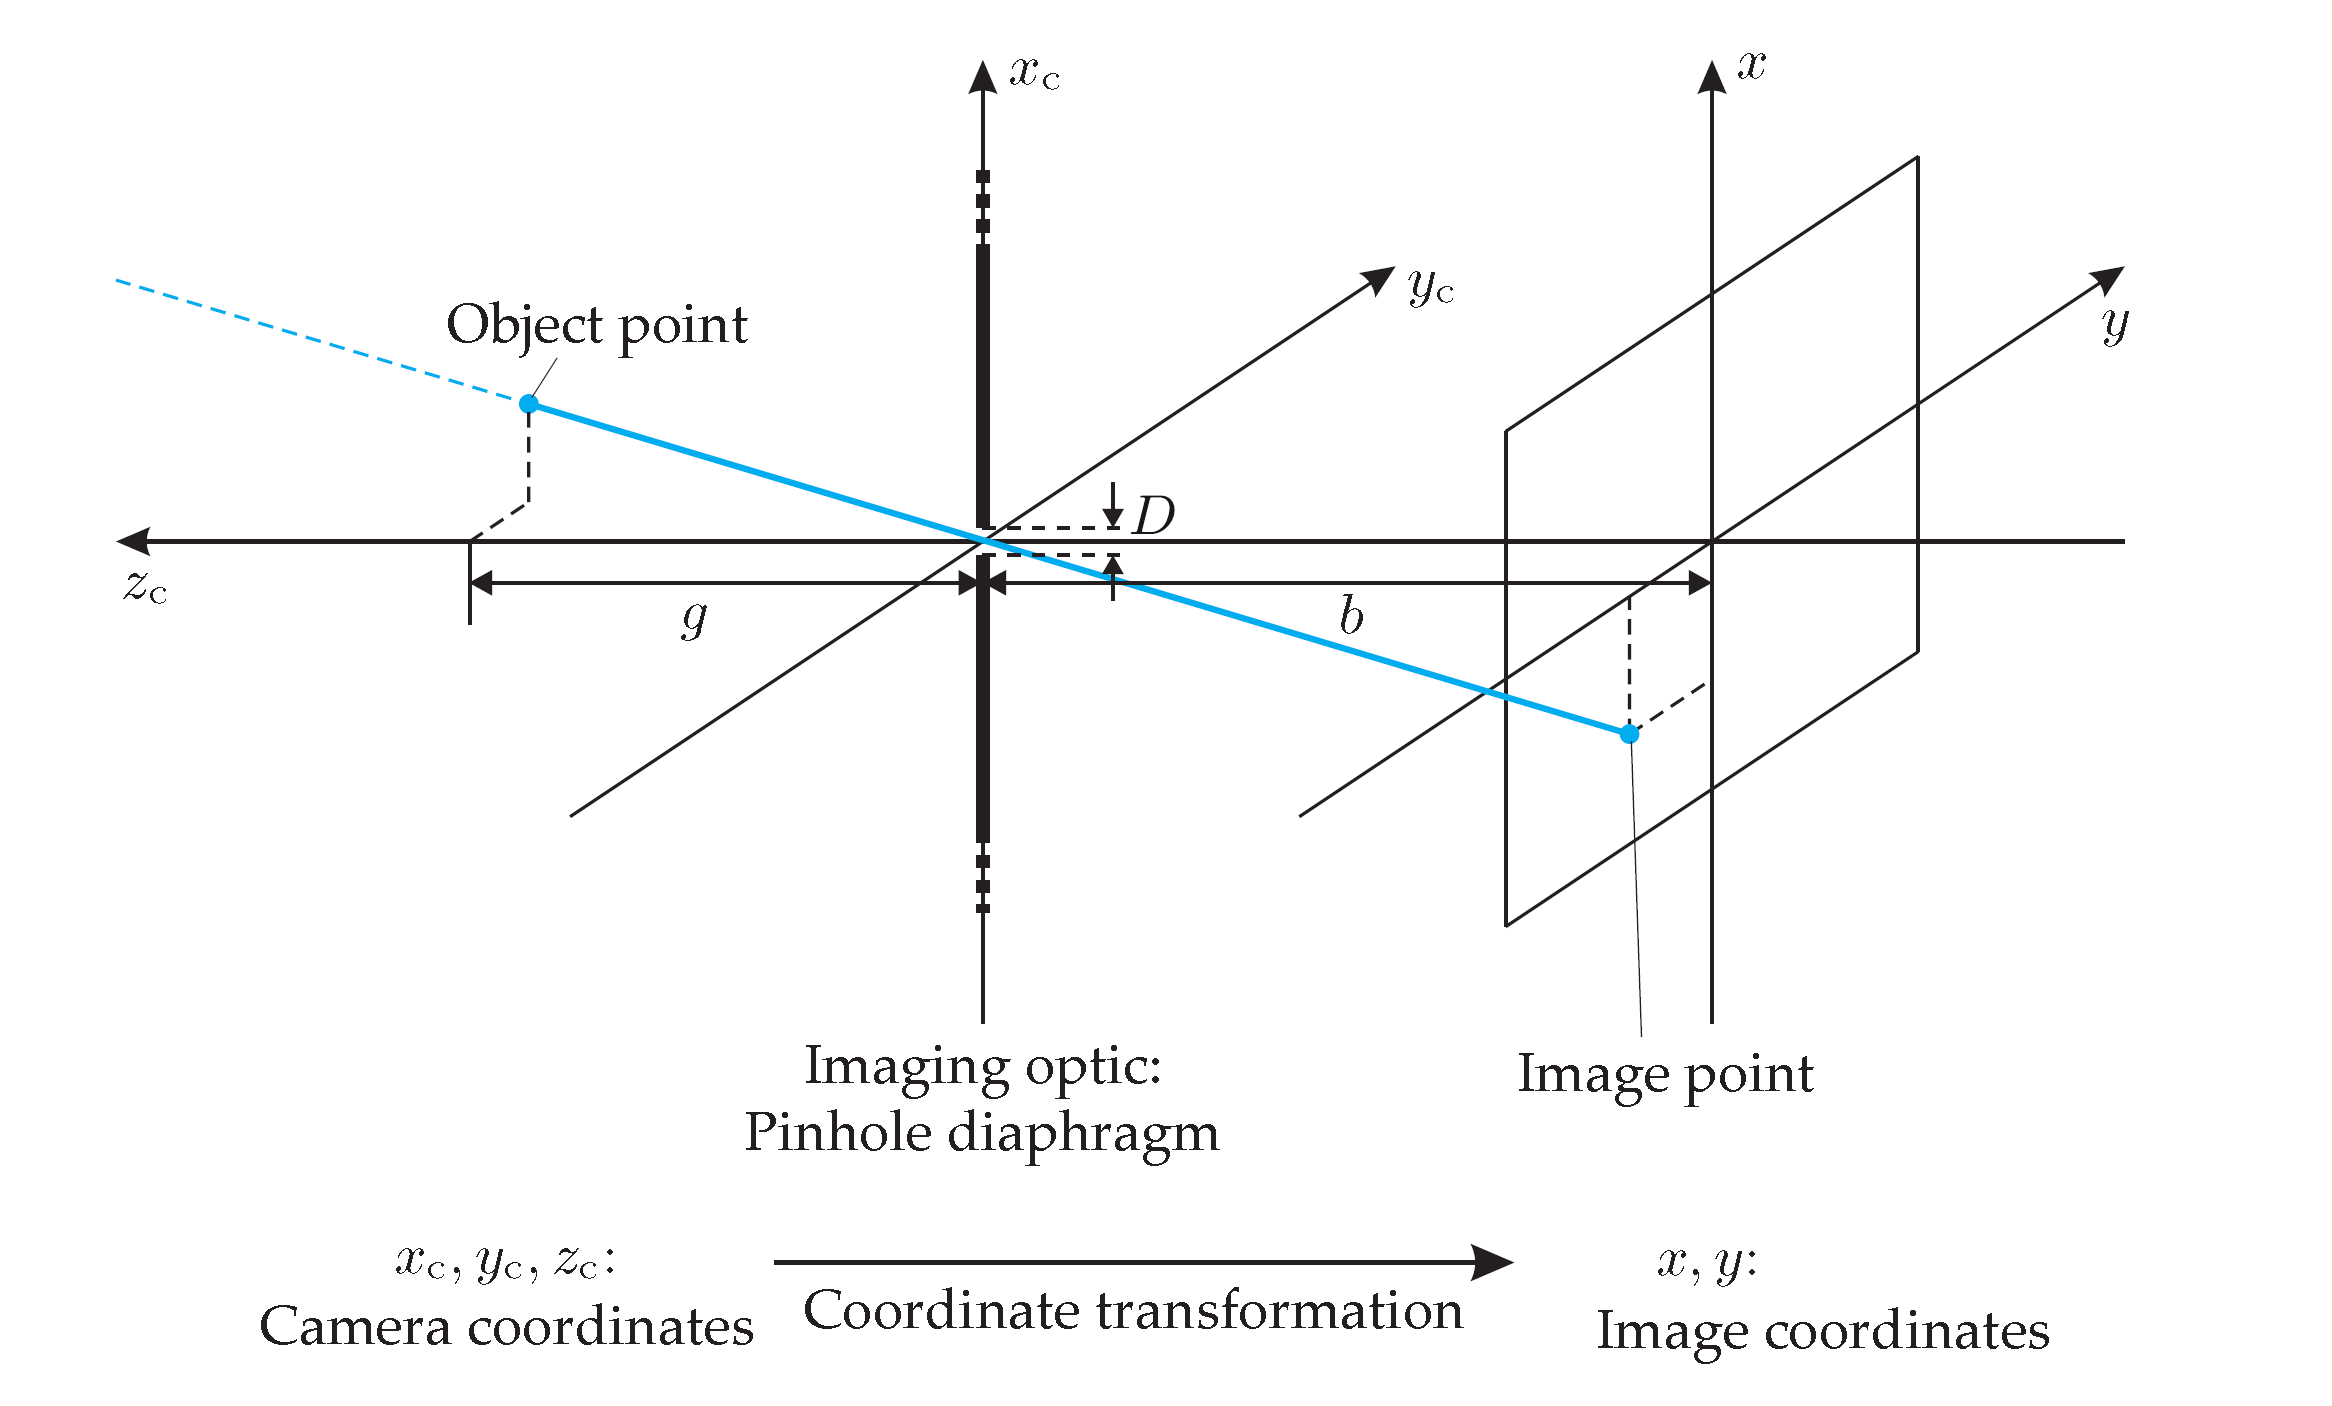
\includegraphics[width=15cm]{images/camera_model.PNG}
\caption{pinhole camera model}
\label{fig:pinhole camera model}
\end{figure}

Before the actual camera model will be explained, we extend the model $x_w$ in \ref{eqn:lf_model1} appropriately. We denote some concept and explain it using the example of pinhole camera. Firstly we denote world coordinate system as $(x_w)$, which defines the position of each object point. The information in this three dimensional world coordinate will be acquisited and imaged in the three dimensional camera coordinate. The transformation from world coordinates to camera coordinates is equivalent to a linear mapping, which can be expressed by a combination of rotation and a subsequent translation transformation:
\begin{equation}
\label{eqn:world-camera transformation}
\begin{pmatrix}
x_c \\
y_c\\
z_c
\end{pmatrix} = \mathrm{R}
\begin{pmatrix}
x_w \\
y_w\\
z_w
\end{pmatrix} + \mathrm{t}
\end{equation}
where $t \in \mathbb{R}_3$ is the translation vector and $\mathbb{R} ∈ \mathbb{R}_{3\times3}$ an orthogonal rotation matrix. Each camera can be characterised as two intrinsic matrices. $\mathrm{C} = [\mathrm{R}\,|\,\mathrm{T}]$.
Until now, the imaging process is still well-defined, unfortunately depth information will be lost when it projected onto image plane, which denoted as $(i_x, i_y)$. Here we just discuss this ill-posed projection process to make the principle clear. The actual camera in the real world can have more completed acquisition process. The distance between the aperture and the image plane is called the image distance $b$. In the case of pinhole camera (Figure \ref{fig:pinhole camera model}), the optical mapping of an object point $x_c$ to an image point $x$ can be mathematically as following:
\begin{equation}
\label{eqn:camera-image transformation}
\begin{pmatrix}
x\\
y\\
\end{pmatrix} = \mathrm{\frac{b}{z_c}}
\begin{pmatrix}
x_c \\
y_c
\end{pmatrix}
\end{equation}
Until now we have introduced the image acquisition process using a simple example. Reconstruct the depth map using integrated light field is a ill-posed problem but not absolutely unsolvable. 





% \subsection{Example: Tables}
% \label{sec:Introduction:Tables}
% \begin{table}
% \centering
% \begin{tabular}{r l}
% \toprule
% abc & def\\
% ghi & jkl\\
% \midrule
% 123 & 456\\
% 789 & 0AB\\
% \bottomrule
% \end{tabular}
% \caption{A table}
% \label{tab:atable}
% \end{table}
\subsection{Disparity and depth estimation}
\label{disparity and depth estimation}

In last section we introduced the theory of imaging process. Depth estimation with single image is without prior knowledge theoretically not possible. An intuitive interpretation for this can be explained through the humanly imaging system. People can not identify the depth and the position of the object using just one eye. This section will introduce the method to estimation the depth using double images. 

In the case of the multi-view images the depth is estimated through the disparity. Mathematically it can be the depth of each pixel well determined by disparity of each, which can be directly derived through geometrical method. We assume that two cameras located at the baseline which is parallel with the optic axis and share the same intrinsic parameter, e.g focal length (Figure \ref{fig:disparity}). Disparity of a given pixel in the image coordinate, denoted as $d$ is defined as the distance moving from left to right view in images, in case of the given Figure  \ref{fig:disparity} is $d=x_1-x_2$. 
Afterwards the depth denoted as $z$ can be derived as following,
where $f$, $x1$, $x_2$, $b$ are given, according to the principle of similar triangles we get:

\begin{figure}
\centering
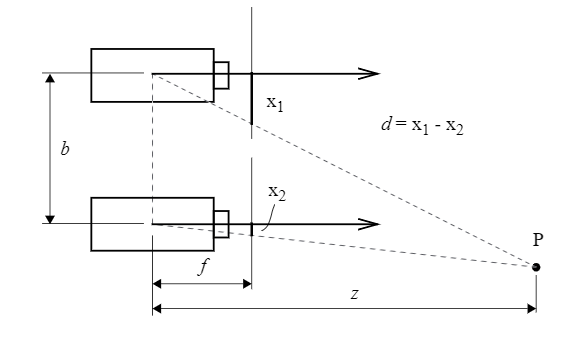
\includegraphics[width=15cm]{images/disparity.PNG}
\caption{disparity of multi-view images system}
\label{fig:disparity}
\end{figure}

\begin{gather}
\label{}
    \frac{z}{f} =  \frac{x}{x_1} \\
    \frac{z}{f} =  \frac{x-b}{x_2}
\end{gather}
where the variable $x$ defines the object's position in the world coordinate in x axis, that is unknown but determined. We solve it for variable $x$ and get: 
\begin{equation}
    x = \frac{b*x_l}{x_l-x_r}
\end{equation}
Finally we get the expression of the depth $z$ with respect to $d$, $f$, $d$.
\begin{equation}
    z = \frac{f*b}{x_l-x_r} = \frac{f*b}{d}
\end{equation}
So far, we have taken the mapping relationship between the disparity and depth. Therefore, the stereo-based depth estimation
methods relied typically on matching pixels across multiple images captured using accurately calibrated cameras. 

\subsection{overview: first and second generation methods}
\label{overview: first and second generation methods}
In section \ref{disparity and depth estimation} we know that the depth estimation relys on the calculation of the disparity. This project's focus is not to implement the conventional method such as SAD, BM, SGBM, GC which are implemented in OpenCV. Understanding these traditional methods give aid to have a basic understanding of existing algorithms, that do not rely on match learning. Futhermore, it can also help us to design an appropriate machine learning algorithms to estimate depth maps. 

\subsubsection{Semi-Global Matching method}
\label{Semi-Global Matching}
This subsection we introduce one of the most popular algorithms Semi-Global Matching. The Semi-Global Matching (SGM) method is based on the idea of pixelwise matching of Mutual Information and approximating a global, 2D smoothness constraint by combining many 1D
constraints\cite{hirschmuller2007stereo}. 


\subsection{summary}

% \begin{displaymath}
% f(x)=\Omega(g(x))\ (x\rightarrow\infty)\;\Leftrightarrow\;
% \limsup_{x \to \infty} \left|\frac{f(x)}{g(x)}\right|> 0
% \end{displaymath}

%% --------------------
%% | /Example content |
%% --------------------